\documentclass{article}

\usepackage{amsmath}
\usepackage{amsthm}
\usepackage{amssymb}
\usepackage{bm}
\usepackage{bbm}
\usepackage{fancyhdr}
% \usepackage{listings}
\usepackage{cite}
\usepackage{graphicx}
\usepackage{enumitem}
\usepackage{courier}
\usepackage[pdftex,colorlinks=true, urlcolor = blue]{hyperref}


\oddsidemargin 0in \evensidemargin 0in
\topmargin -0.5in \headheight 0.25in \headsep 0.25in
\textwidth 6.5in \textheight 9in
\parskip 6pt \parindent 0in \footskip 20pt

% set the header up
\fancyhead{}
\fancyhead[L]{Stanford Aeronautics \& Astronautics}
\fancyhead[R]{Fall 2020}

%%%%%%%%%%%%%%%%%%%%%%%%%%
\renewcommand\headrulewidth{0.4pt}
\setlength\headheight{15pt}

\usepackage{xparse}
\NewDocumentCommand{\codeword}{v}{%
\texttt{\textcolor{blue}{#1}}%
}

\usepackage{xcolor}
\setlength{\parindent}{0in}

\title{AA 274A: Principles of Robot Autonomy I \\ Problem Set X}
\author{Name: Li Quan Khoo     \\ SUID: lqkhoo (06154100)}
\date{}

\begin{document}

\maketitle
\pagestyle{fancy} 

\section*{Problem 1: Trajectory Generation via Differential Flatness}
\begin{enumerate}[label=(\roman*)]
\item % (i)

We are given initial and final conditions in terms of variables $\{x, y, V, \theta\}$. The equations are:

$$
\begin{bmatrix}
1 & 0   & 0      & 0 \\
0 & 1   & 0      & 0 \\
1 & t_f & t_f^2  & t_f^3 \\
0 & 1   & 2 t_f  & 3 t_f^2
\end{bmatrix}
\begin{bmatrix}
x_1 \\ x_2 \\ x_3 \\ x_4
\end{bmatrix}
=
\begin{bmatrix}
x(0) \\ \dot{x}(0) \\ x(t_f) \\ \dot{x}(t_f)
\end{bmatrix}
$$

$$
\begin{bmatrix}
1 & 0   & 0      & 0 \\
0 & 1   & 0      & 0 \\
1 & t_f & t_f^2  & t_f^3 \\
0 & 1   & 2 t_f  & 3 t_f^2
\end{bmatrix}
\begin{bmatrix}
y_1 \\ y_2 \\ y_3 \\ y_4
\end{bmatrix}
=
\begin{bmatrix}
y(0) \\ \dot{y}(0) \\ y(t_f) \\ \dot{y}(t_f)
\end{bmatrix}
$$

where $\dot{x}(t)=V\cos\theta$ and $\dot{y}(t)=V\sin\theta$ as given by the robot's kinematic model.


\item % (ii)
Since $\det(\bm{J})=V$, $V>0\; \forall t$ is a sufficient and necessary condition for the matrix $\bm{J}$ to be invertible.

\item % (iii)
(code)

\item % (iv)
(code)

\item % (v)
\begin{tabular}[t]{c}
	\hline \\
	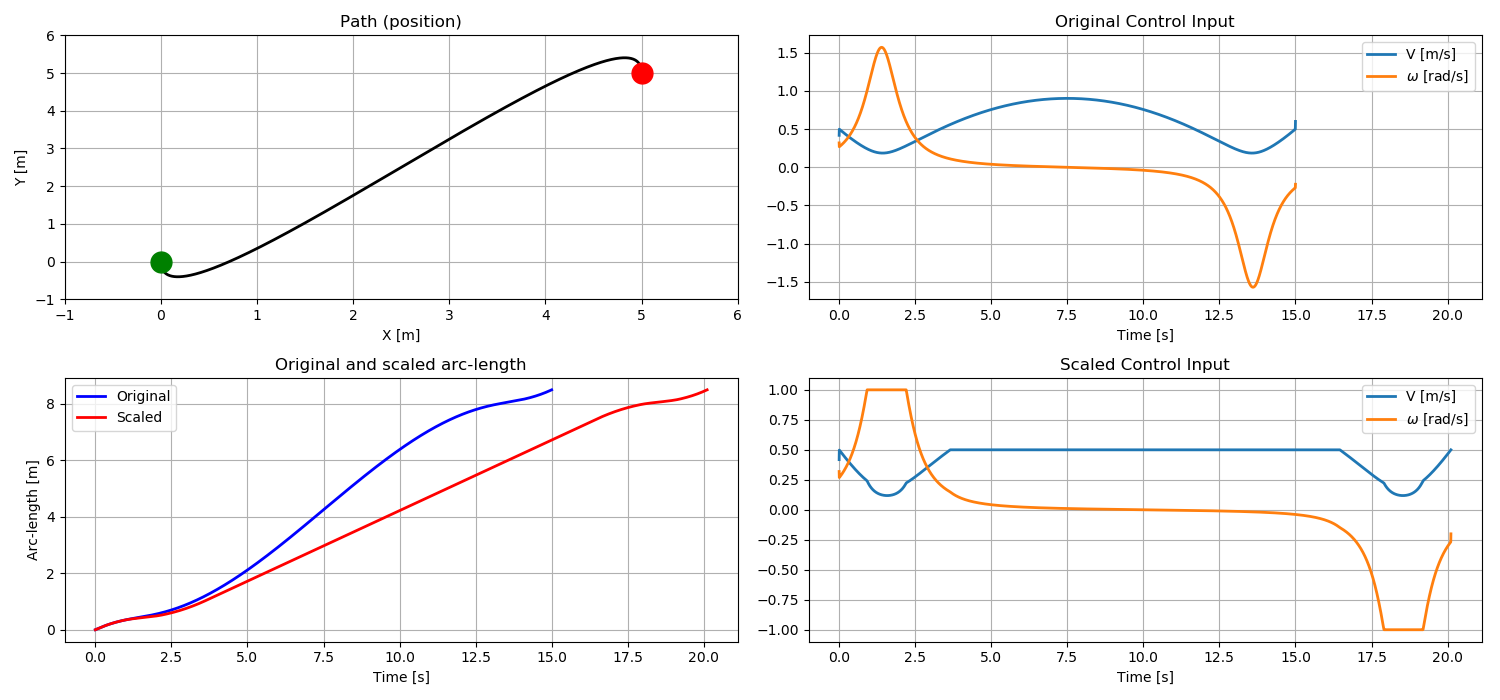
\includegraphics[width=1.0\textwidth]{img/differential_flatness.png} \\
	Trajectory of unicycle model in absence of noise. Initial and final conditions as given. \\
	\hline
\end{tabular}

\item % (vi)
\begin{tabular}[t]{c}
	\hline \\
	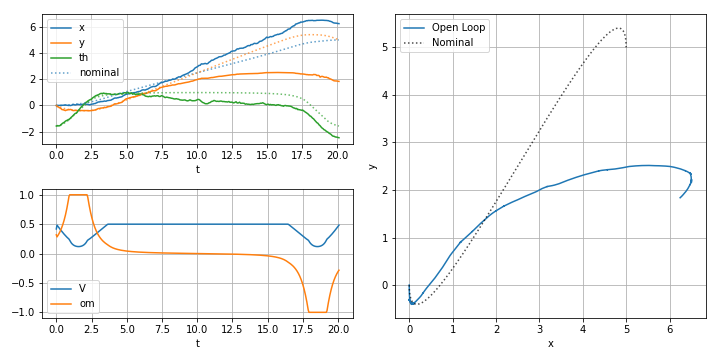
\includegraphics[width=1.0\textwidth]{img/sim_traj_openloop.png} \\
	Trajectory of unicycle model where control vector $u_\text{noisy}=u + \epsilon$ where $\epsilon$ is simulated isotropic Gaussian noise. \\
	\hline
\end{tabular}


\end{enumerate}

\section*{Problem 2: Pose Stabilization}

	\begin{enumerate}[label=(\roman*)]
		
	\item % (i)
	(code)
	
	\item % (ii)
	(code)
	
	\item % (iii)
	\begin{tabular}[t]{c}
		\hline \\
		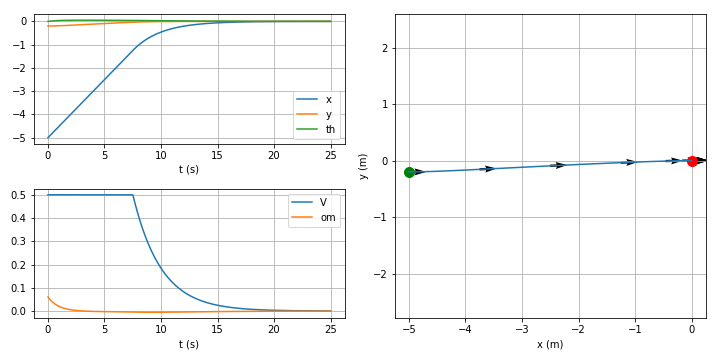
\includegraphics[width=1.0\textwidth]{img/sim_parking_forward.png} \\
		Forward parking \\
		\hline
	\end{tabular}
	\begin{tabular}[t]{c}
		\hline \\
		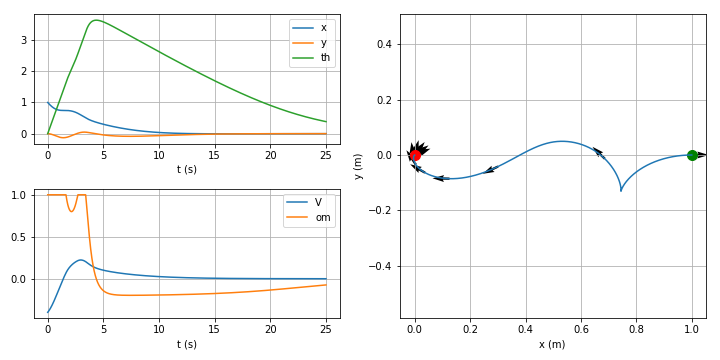
\includegraphics[width=1.0\textwidth]{img/sim_parking_reverse.png} \\
		Reverse parking \\
		\hline
	\end{tabular}
	\begin{tabular}[t]{c}
		\hline \\
		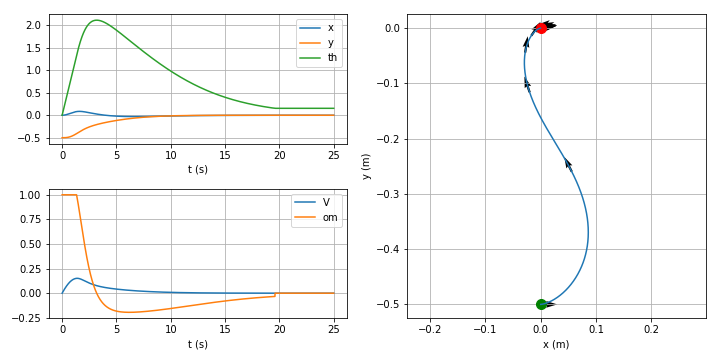
\includegraphics[width=1.0\textwidth]{img/sim_parking_parallel.png} \\
		Parallel parking \\
		\hline
	\end{tabular}
		
	\end{enumerate}

\pagebreak

\section*{Problem 3: Trajectory Tracking}

	\begin{enumerate}[label=(\roman*)]
	
	\item % (i)
	Starting from our extended unicycle model, the given kinematic equations are:
	
	\begin{equation}
	\begin{aligned}
	\dot{x}(t) &= V\cos(\theta) \\
	\dot{y}(t) &= V\sin(\theta) \\
	\dot{V}(t) &= a(t) \\
	\dot{\theta}(t) &= \omega(t)
	\end{aligned}
	\end{equation}
	
	\begin{equation}
	\underbrace{
		\begin{bmatrix}
		\ddot{x}(t) \\
		\ddot{y}(t)
		\end{bmatrix}
	}_{\ddot{\bm{z}}=\bm{z}^{(q+1)}}
	=
	\underbrace{
		\begin{bmatrix}
		\cos(\theta) & -V\sin(\theta) \\
		\sin(\theta) & V\cos(\theta) \\
		\end{bmatrix}
	}_{:=\bm{J}}
	\begin{bmatrix}
	a \\
	\omega
	\end{bmatrix}
	:=
	\underbrace{
		\begin{bmatrix}
		u_1 \\
		u_2
		\end{bmatrix}
	}_{\bm{w}}
	\end{equation}
	
	Equation (2) is in the form of a linear ODE $\bm{z}^{(q+1)}=\bm{w}$. For the unicycle model, $q$ is known to be 1. We want to design a control law for the virtual input term $\bm{w}$.
	
	Below is the exact linearization scheme in lecture 4. Where superscript $(j)$ denotes the jth derivative w.r.t. $t$, subscript $d$ denotes the 'desired' open-loop trajectory that we wish to track, we define $i$th component of the linear tracking error to be:
	
	\begin{equation}
	\begin{aligned}
	e_i(t) &:=z_i(t) - z_{i,d}(t) \\
	e_i^{(q+1)}(t) &= z^{(q+1)}_i(t) - z^{(q+1)}_{i,d}(t) \\
	               &= w_i - w_{i,d} \\
	\bm{e}(t) &= \bm{w}(t) - \bm{w}_d(t)
	\end{aligned}
	\end{equation}
	, which is a second-order ODE for our system.
	
	Following lecture 4 notes, we consider a closed-loop control law of the form:
	
	\begin{equation}
	w_i(t) = w_{i,d}(t) - \sum_{j=0}^q k_{i,j}e_i^{(j)}(t)
	\end{equation}
	
	which results in closed-loop dynamics of the form:
	
	\begin{equation}
	\bm{z}^{(q+1)} = \bm{w}_d - \sum_{j=0}^q K_j \bm{e}^{(j)}
	\end{equation}
	
	, where $K_j$ is a diagonal matrix containing elements $k_{i,j}$. Since $\bm{z}_d^{(q+1)}=\bm{w}_d$, we finally get:
	
	\begin{equation}
	\bm{e}^{(q+1)} + \sum_{j=0}^q K_j \bm{e}^{(j)} = 0
	\end{equation}
	
	For our system, (6) becomes:
	
	\begin{equation}
	\begin{aligned}
	(\ddot{x}-\ddot{x}_d) &+ k_{dx}(\dot{x} - \dot{x}) &+ k_{px}(x_d - x) = 0 \\
	\underbrace{(\ddot{y}-\ddot{y}_d)}_{\ddot{e}} &+
	k_{dy}\underbrace{(\dot{y} - \dot{y})}_{\dot{e}} &+
	k_{py}\underbrace{(y_d - y)}_{e} = 0
	\end{aligned}
	\end{equation}
	
	This is a 2nd order ODE in $\bm{e}$ in standard form. We know that for the system to be stable, the real parts of both roots of its characteristic equation must be $>0$. We also know that the system is critically-damped when the roots are equal. This tells us what the values of $K$ should be.
	
	Rearranging (7), since $\ddot{x}=u_1$ and $\ddot{y}=u_2$ from (2), we get:
	
	\begin{equation}
	\begin{aligned}
	u_1 &= \ddot{x}_d &+ k_{px}(x_d - x) &+ k_{dx}(\dot{x} - \dot{x}) = 0 \\
	u_2 &= \ddot{y}_d &+ k_{py}(y_d - y) &+ k_{dy}(\dot{y} - \dot{y}) = 0
	\end{aligned}
	\end{equation}
	
	Finally, to recover our real controls $\{a, \omega\}$, we invert $J$ in (2) and solve for:

	\begin{equation}
	\begin{aligned}
	\begin{bmatrix}
	a \\
	w
	\end{bmatrix}
	&=
	J^{-1}
	\begin{bmatrix}
	u_1 \\
	u_2
	\end{bmatrix} \; , \; V>0 \\
	\begin{bmatrix}
	a \\
	w
	\end{bmatrix}
	&=
	\frac{1}{V}
	\begin{bmatrix}
	V\cos(\theta) & V\sin(\theta) \\
	-\sin(\theta) & \cos(\theta)
	\end{bmatrix}
	\begin{bmatrix}
	u_1 \\
	u_2
	\end{bmatrix}
	\end{aligned}
	\end{equation}
	
	To recover $V$ as the problem requested,
	
	\begin{equation}
	\begin{aligned}
	V(T) &= \int_{t_0}^T a(t) \; dt \\
	V_t &= V_{t-1} + a_t \Delta t
	\end{aligned}
	\end{equation}
	
	\item % (ii)
	(code)
	
	\item % (iii)
	\begin{tabular}[t]{c}
	\hline \\
	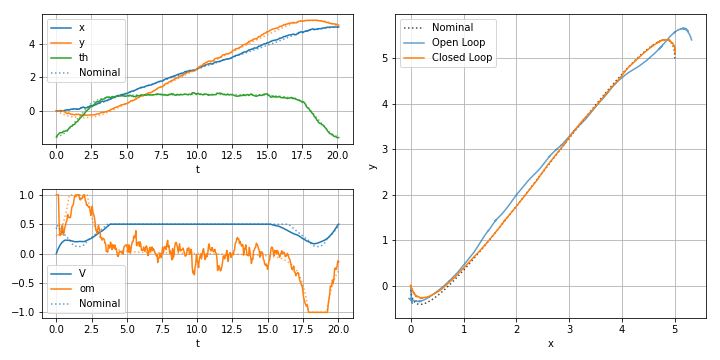
\includegraphics[width=1.0\textwidth]{img/sim_traj_closedloop.png} \\
	Trajectory of unicycle under two-part tracking controller. \\
	\hline
	\end{tabular}
	
	\end{enumerate}

\pagebreak

\section*{Extra Problem: Optimal Control and Trajectory Optimization}

	\begin{enumerate}[label=(\roman*)]
	
	\item % (i)
	To minimize:
	\begin{equation}
	J = \int_0^{t_f} \underbrace{[\lambda + V^2 + \omega^2]}_{g} dt \;,\;\; \lambda \; \text{constant}
	\end{equation}
	
	Subject to:
	\begin{equation}
	\begin{aligned}
	\dot{x} &= V\cos\theta \\
	\dot{y} &= V\sin\theta \\
	\dot{\theta} &= \omega
	\end{aligned}
	\end{equation}
	
	Boundary conditions:
	\begin{equation}
	{\renewcommand{\arraystretch}{1.4}
	\begin{tabular}[c]{c c c}
		$x(0) = 0$ & $y(0) = 0$ & $\theta(0)$ = $-\frac{\pi}{2}$ \\
		$x(t_f) = 5$ & $y(t_f) = 5$ & $\theta(t_f) = -\frac{\pi}{2}$
	\end{tabular}}
	\end{equation}
	
	\hrulefill
	
	We follow the procedure outlined in lecture 5.
	
	Let:
	\begin{equation}
	\dot{\bm{x}} =
	\begin{bmatrix}
	\dot x \\
	\dot y \\
	\dot \theta
	\end{bmatrix} \; , \;
	\bm{u} = 
	\begin{bmatrix}
	V \\
	\omega
	\end{bmatrix} \; , \;
	\bm f = 
	\begin{bmatrix}
	V\cos\theta \\
	V\sin\theta \\
	\omega
	\end{bmatrix}
	\end{equation}
	
	1. First, we need the Hamiltonian for the system:
	\begin{equation}
	\begin{aligned}
	\mathcal{H} &= g + \bm p^\mathsf{T} \bm f \\
	\mathcal{H} &= \lambda + V^2 + \omega^2 +
	               p_1 V\cos\theta + p_2 V\sin\theta + p_3 \omega
	\end{aligned}
	\end{equation}
	
	2. Next, we find the NOCs, which are defined by:
	\begin{equation}
	\begin{aligned}
	\dot{\bm{x}}^* &= \frac{\partial \mathcal{H}}{\partial \bm{p}} \\
	\dot{\bm{p}}^* &= -\frac{\partial \mathcal{H}}{\partial \bm{x}} \\
	0 &= \frac{\partial \mathcal{H}}{\partial \bm{u}}
	\end{aligned}
	\end{equation}
	
	For our system, these correspond to $2n+m$ equations. To solve for $t_f$, we additionally define a dummy state variable $r$ such that $r=t_f$ and $\dot r=0$.
	
	The NOCs for our system are:
	
	\begin{equation}
	{\renewcommand{\arraystretch}{1.4}
	\begin{tabular}[c]{l l l l l}
	$\dot x^* = V \cos\theta$ &\;&
	$\dot p_1^* = 0$	&\;&
	$0 = \frac{\partial\mathcal{H}}{\partial V}$ \\
	
	$\dot y^* = V \sin\theta$ &\;&
	$\dot p_2^* = 0$	&\;&
	$0 = \frac{\partial\mathcal{H}}{\partial \omega}$ \\
	
	$\dot \theta^* = \omega$ &\;&
	$\dot p_3^* = p_1V\sin(\theta) - p_2V\cos(\theta)$ \\
	
	$\dot r^* = 0$
	\end{tabular}}
	\end{equation}
	
	Since
	\begin{equation}
	\begin{aligned}
	\frac{\partial\mathcal{H}}{\partial \omega} = 2\omega + p_3 &= 0 \quad,\quad \frac{\partial\mathcal{H}}{\partial V} = 2V + p_1\cos(\theta) + p_2\sin(\theta) \\
	\omega &=-\frac{p_3}{2} \quad,\quad V = -\frac{p_1\cos(\theta)+p_2\sin(\theta)}{2}
	\end{aligned}
	\end{equation}
	
	\pagebreak
	
	3. We need to have $2n+1$ boundary conditions to solve for the $2n$ differential equations plus 1 free variable $t_f$. With $x_f$ fixed and $t_f$ free, these are governed by:
	
	\begin{equation}
	\begin{aligned}
	x^*(t_0) &= x_0 \\
	x^*(t_f) &= x_f \\
	\mathcal{H} + \frac{\partial h}{\partial t} &= 0
	\end{aligned}
	\end{equation}
	
	In our case, $h=0$ as we don't have initial cost. These correspond to:
	\begin{equation}
	\begin{aligned}
	&{\renewcommand{\arraystretch}{1.4}
	\begin{tabular}[c]{l l l}
	$x^*(0) = 0$ & $x^*(t_f) = 5$ \\
	$y^*(0) = 0$ & $y^*(t_f) = 5$ \\
	$\theta^*(0) = -\frac{\pi}{2}$ & $\theta^*(t_f) = -\frac{\pi}{2}$ \\
	\end{tabular}} \\
	&\lambda + V^2 + \omega^2 + p_1 V\cos\theta + p_2 V\sin\theta + p_3 \omega = 0
	\end{aligned}
	\end{equation}
	
	4. Now we need to rescale for time. Let $\tau$ be our new time scale such that:
	\begin{equation}
	\begin{aligned}
	\tau &= \frac{t}{t_f} \;,\; \tau \in [0,1] \\
	\frac{d}{d\tau} &= \frac{dt}{d\tau} \cdot \frac{d}{dt}   = t_f \frac{d}{dt}
	\end{aligned}
	\end{equation}
	
	Denoting $\frac{d}{d\tau}$ as $[.]'$, the NOCs become:
	
	\begin{equation}
	{\renewcommand{\arraystretch}{1.4}
	\begin{tabular}[c]{l l l l l}
	$x^{'*} = rV \cos\theta$ 	&\;&
	$p_1^{'*} = 0$	&\;&
	$0 = \frac{\partial\mathcal{H}}{\partial V}$ \\
	
	$y^{'*} = rV \sin\theta$ 	&\;&
	$p_2^{'*} = 0$	&\;&
	$0 = \frac{\partial\mathcal{H}}{\partial \omega}$ \\
	
	$\theta^{'*} = r\omega$ &\;&
	$p_4^{'*} = rp_1V\sin(\theta) - rp_2V\cos(\theta)$ \\
	
	$r^{'*} = 0$
	\end{tabular}}
	\end{equation}
	
	The boundary conditions do not have $t$ terms, so the expressions remain the same.
	
	\item % (ii)
	(code)
	
	\item % (iii)
	\begin{tabular}[t]{c}
		\hline \\
		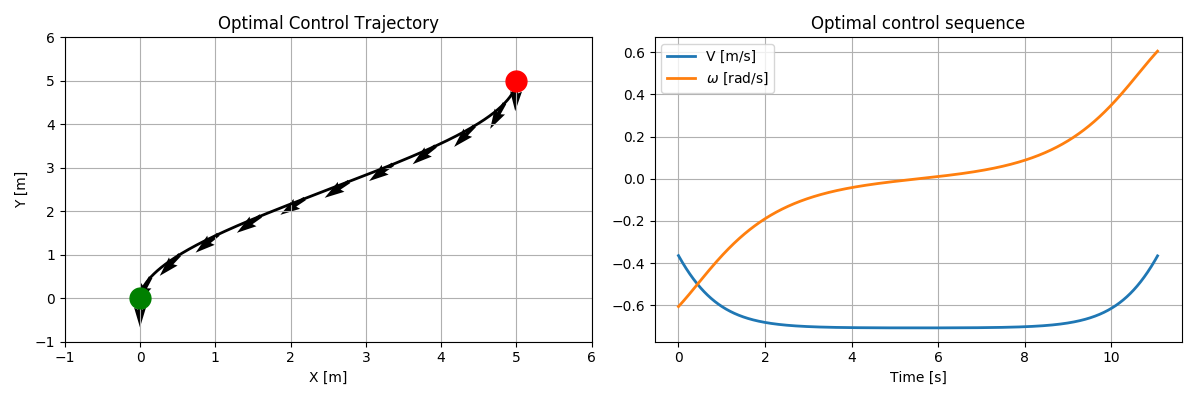
\includegraphics[width=1.0\textwidth]{img/optimal_control.png} \\
		Trajectory of unicycle model as solved by nonlinear optimization.\\
		\hline
	\end{tabular}
	
	\item % (iv)
	The larger $\lambda$ is, the larger the emphasis the solver puts on minimizing time.

	\pagebreak

	\item % (v)
	\begin{tabular}[t]{c}
		\hline \\
		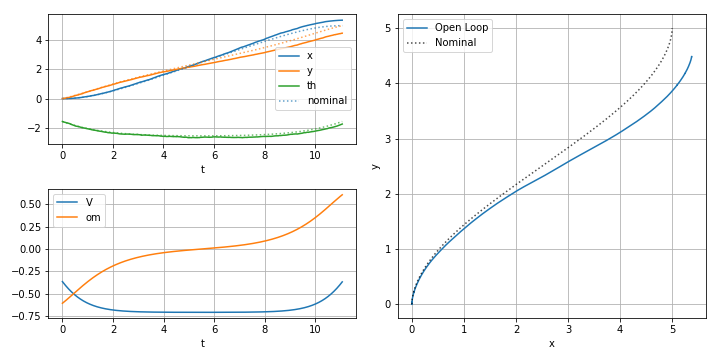
\includegraphics[width=1.0\textwidth]{img/sim_traj_optimal_control.png} \\
		Comparison of open-loop trajectory and optimized trajectory in presence of isotropic Gaussian noise. \\
		\hline
	\end{tabular}
	
	
	\end{enumerate}

\end{document}
